\section{Anhang}
\label{sec:Anhang}
\subsection{Originaldaten}
\centering
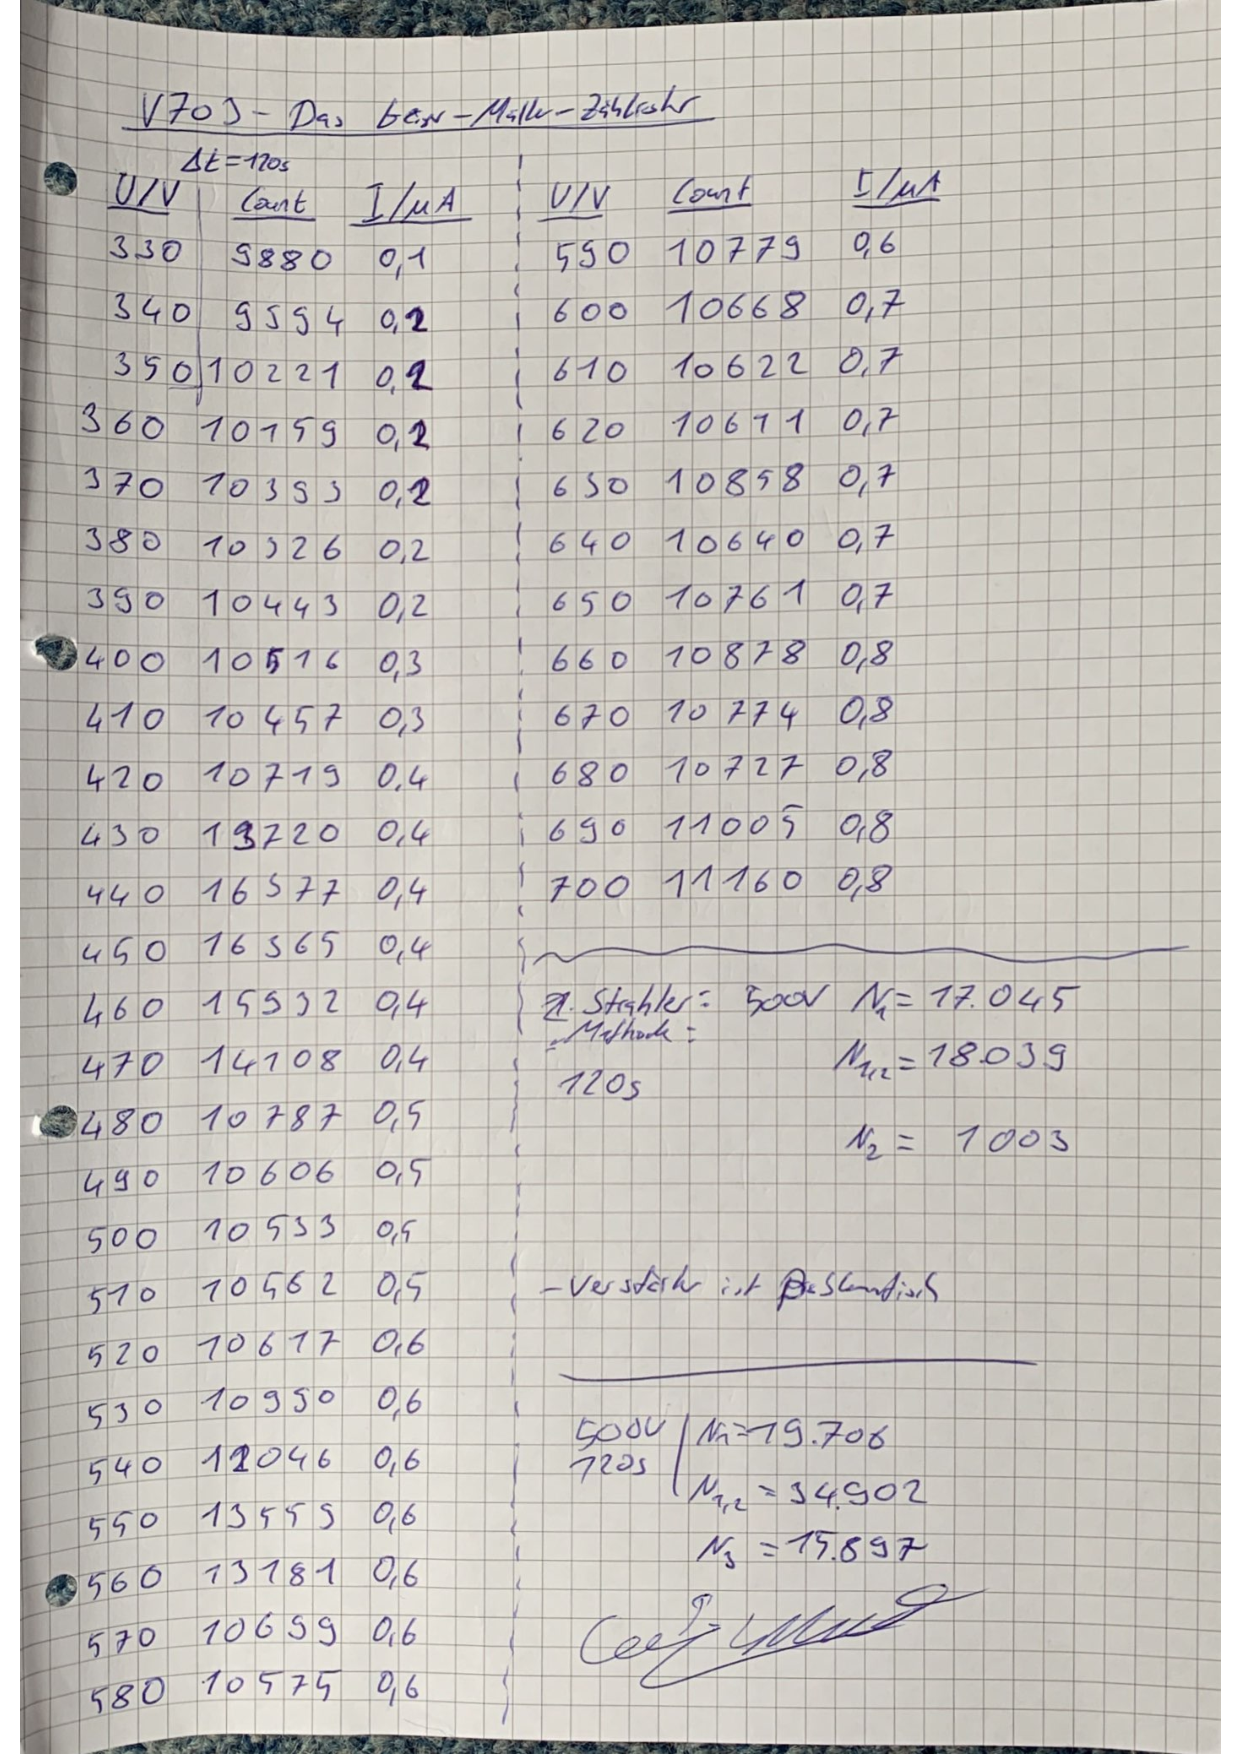
\includegraphics[height=18cm]{content/pics/originaldaten/Originaldaten_1.pdf}
% \newpage
% \centering
% 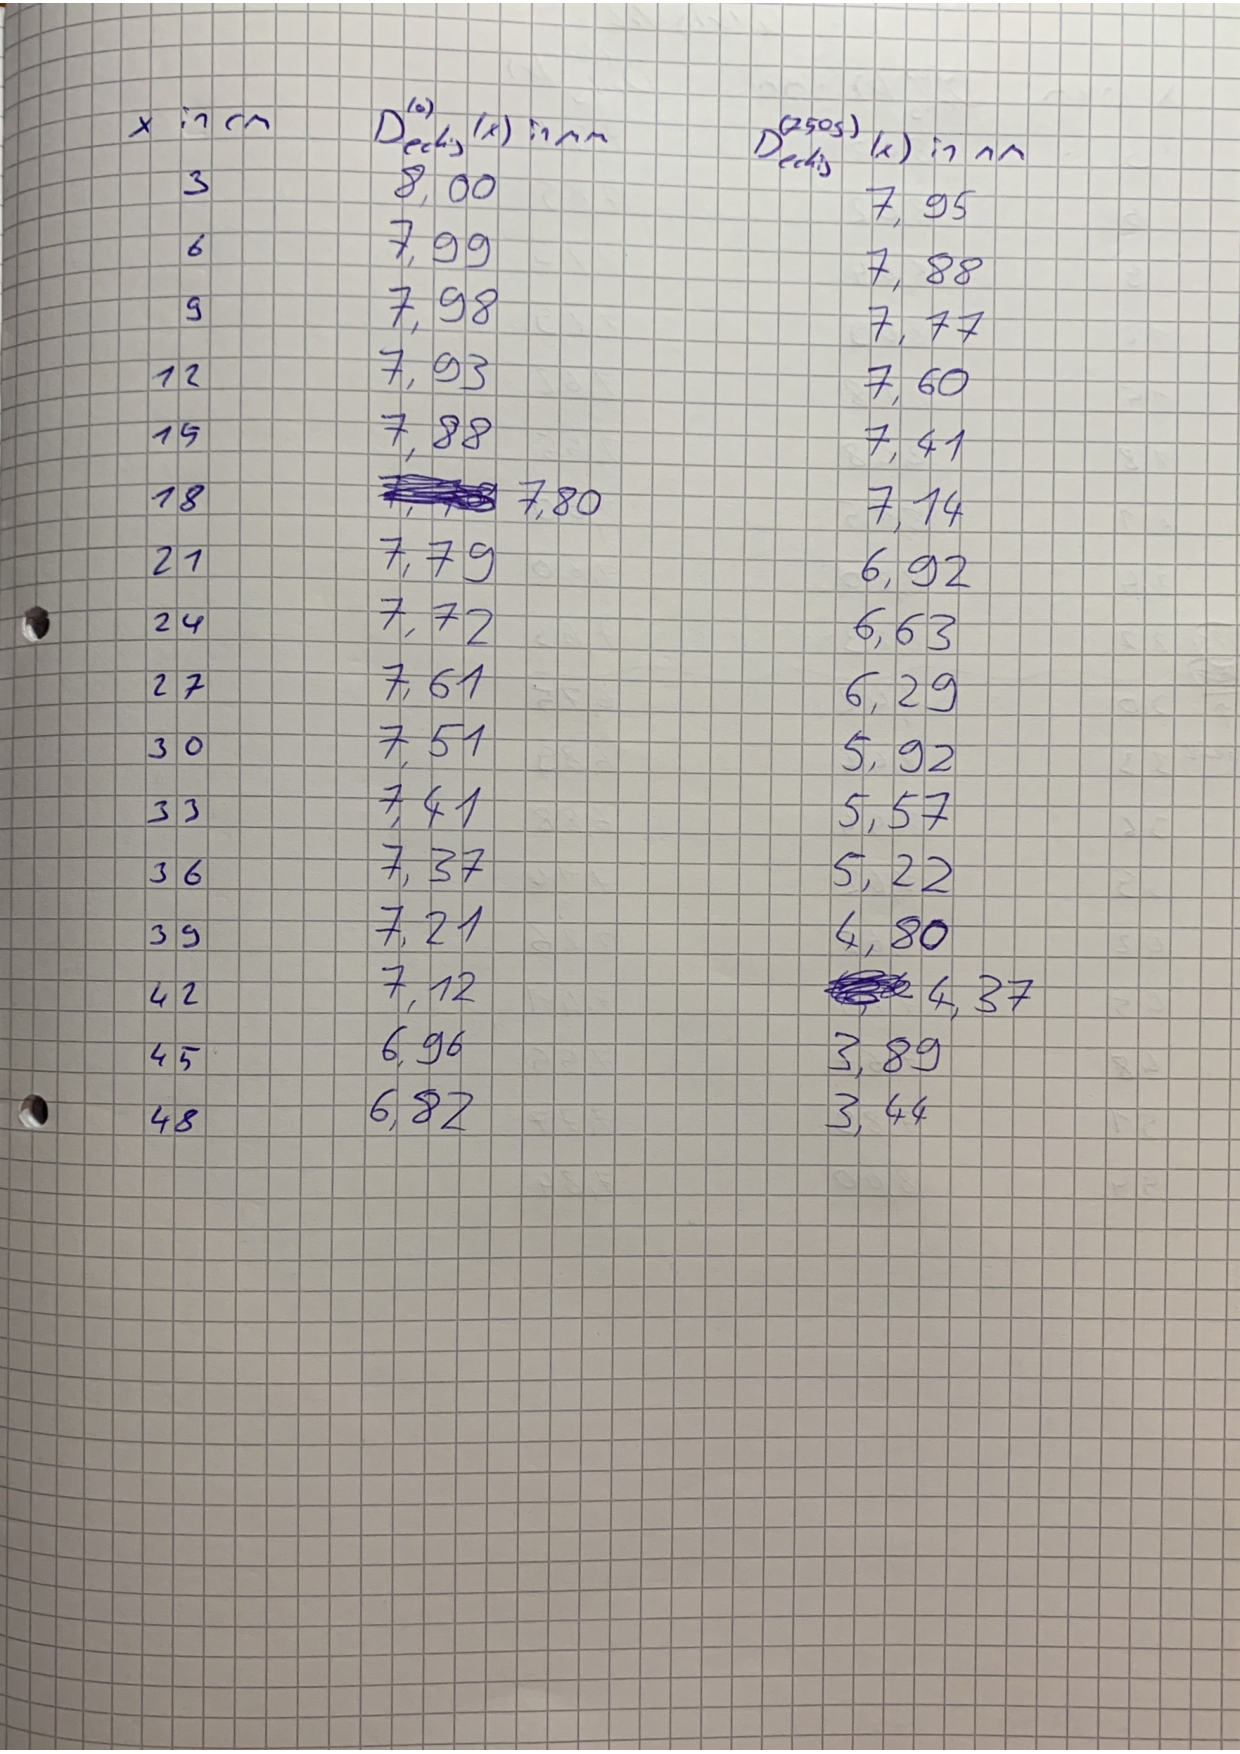
\includegraphics[height=18cm]{content/pics/originaldaten/Originaldaten_2.pdf}
% \newpage
% \centering
% 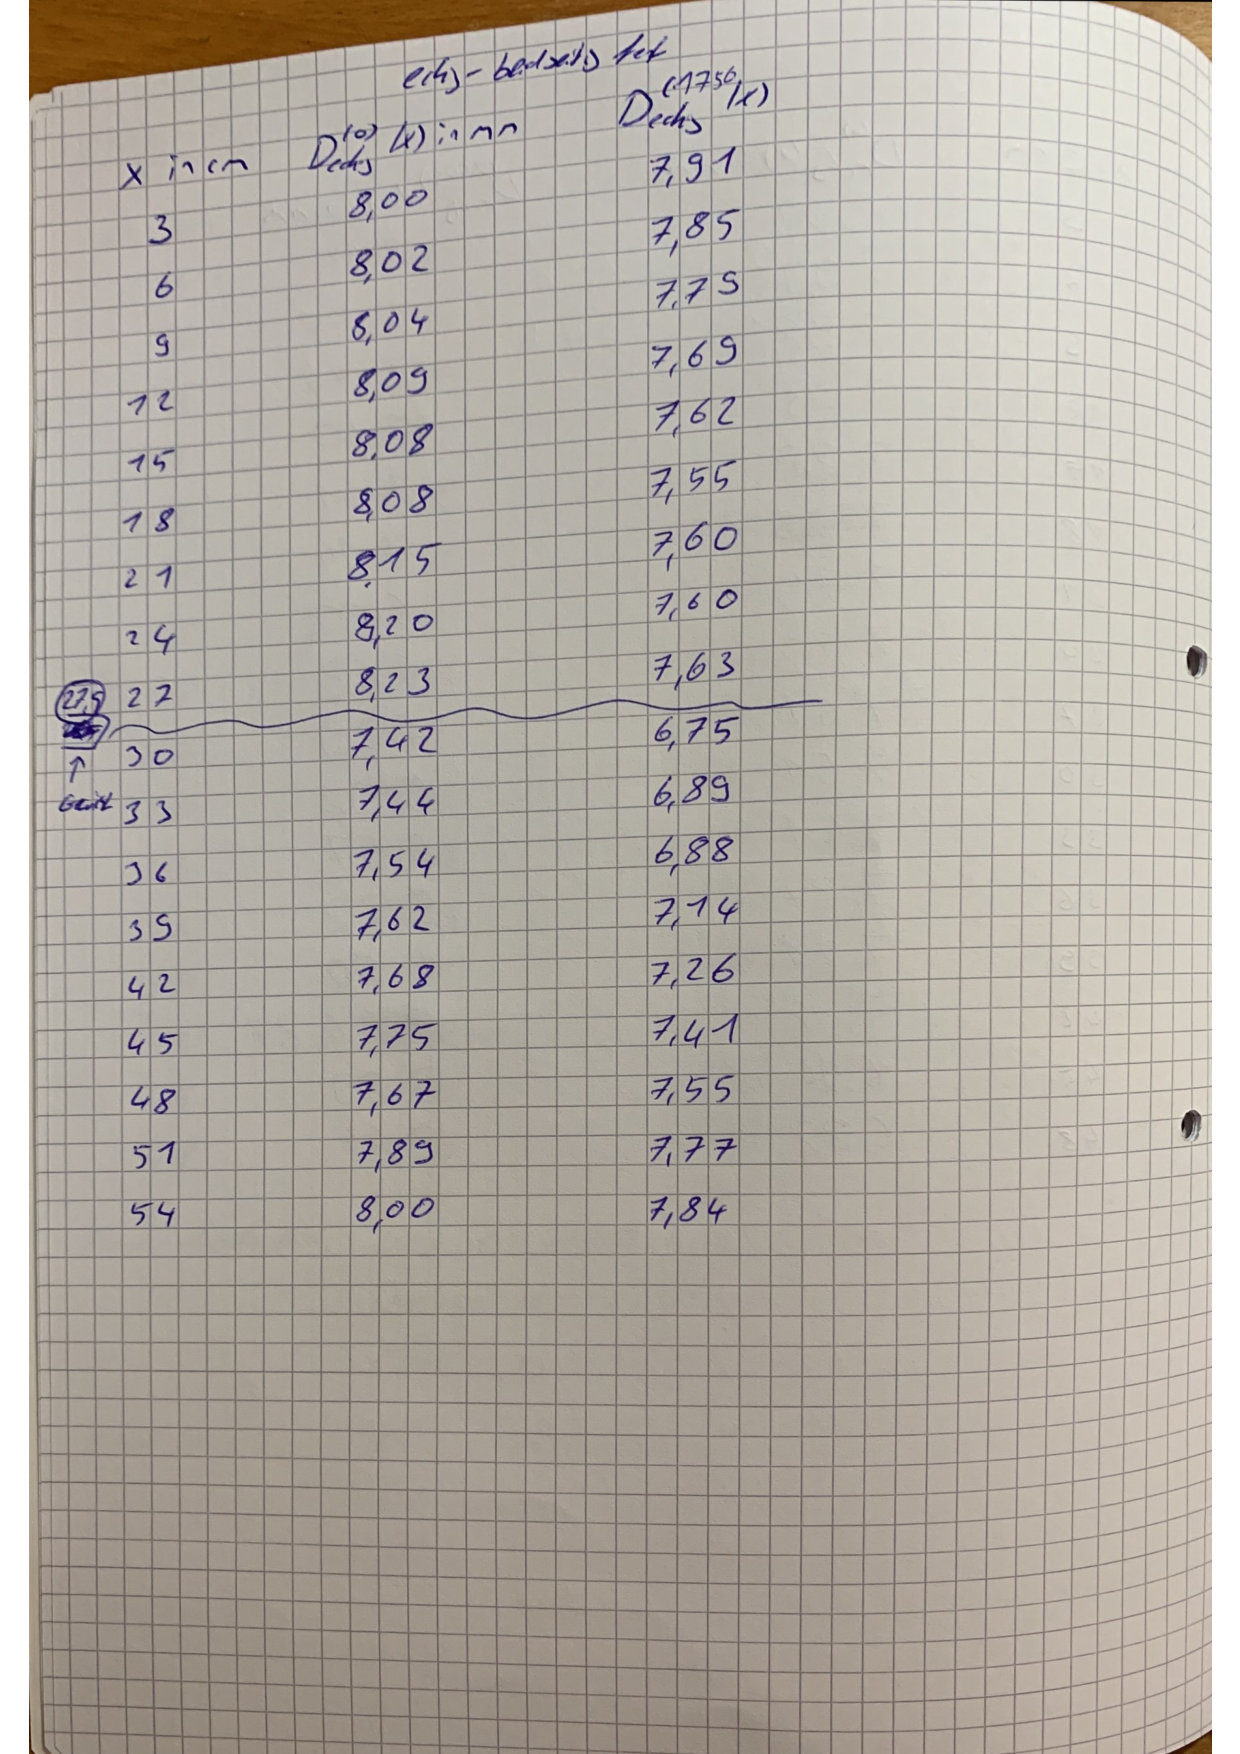
\includegraphics[height=18cm]{content/pics/originaldaten/Originaldaten_3.pdf}
% \newpage
% \centering
% 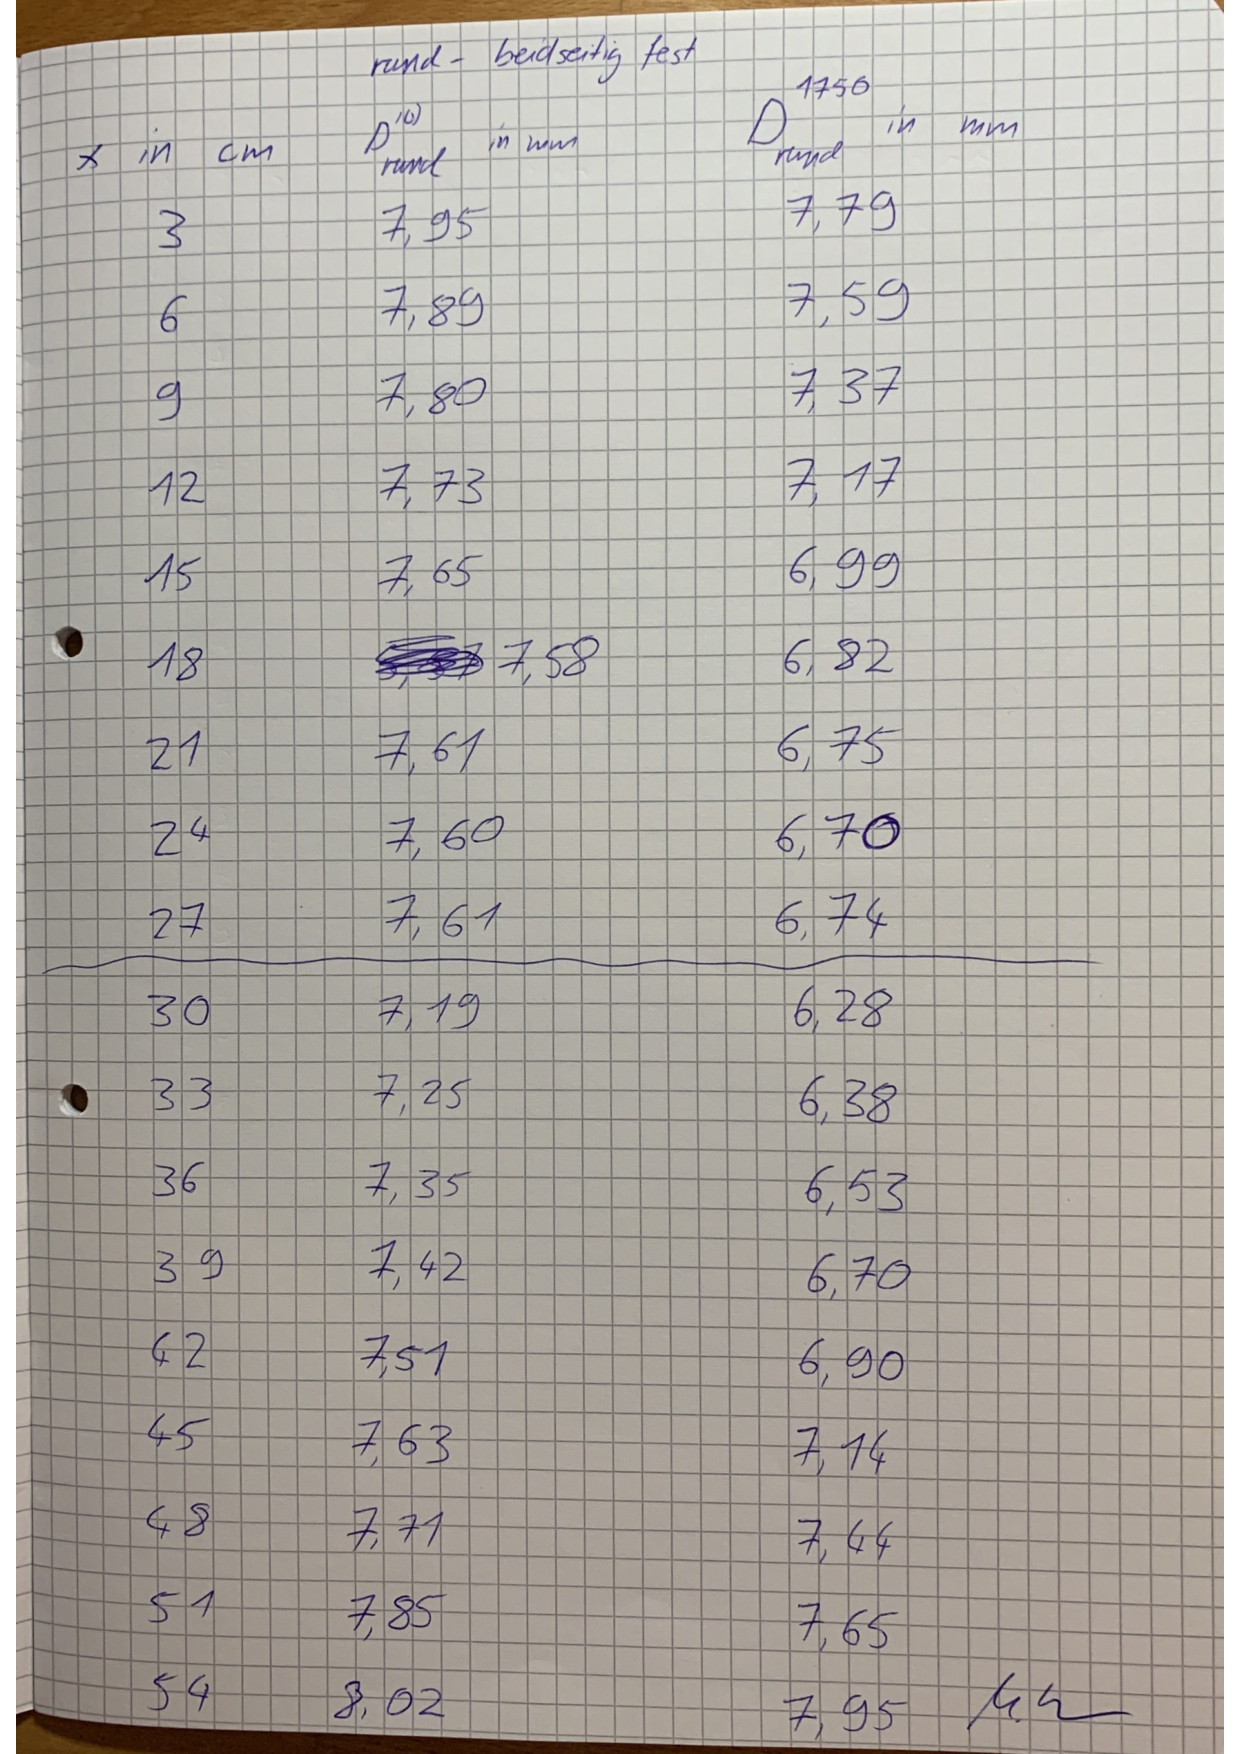
\includegraphics[height=18cm]{content/pics/originaldaten/Originaldaten_4.pdf}
% \newpage
% \centering
% 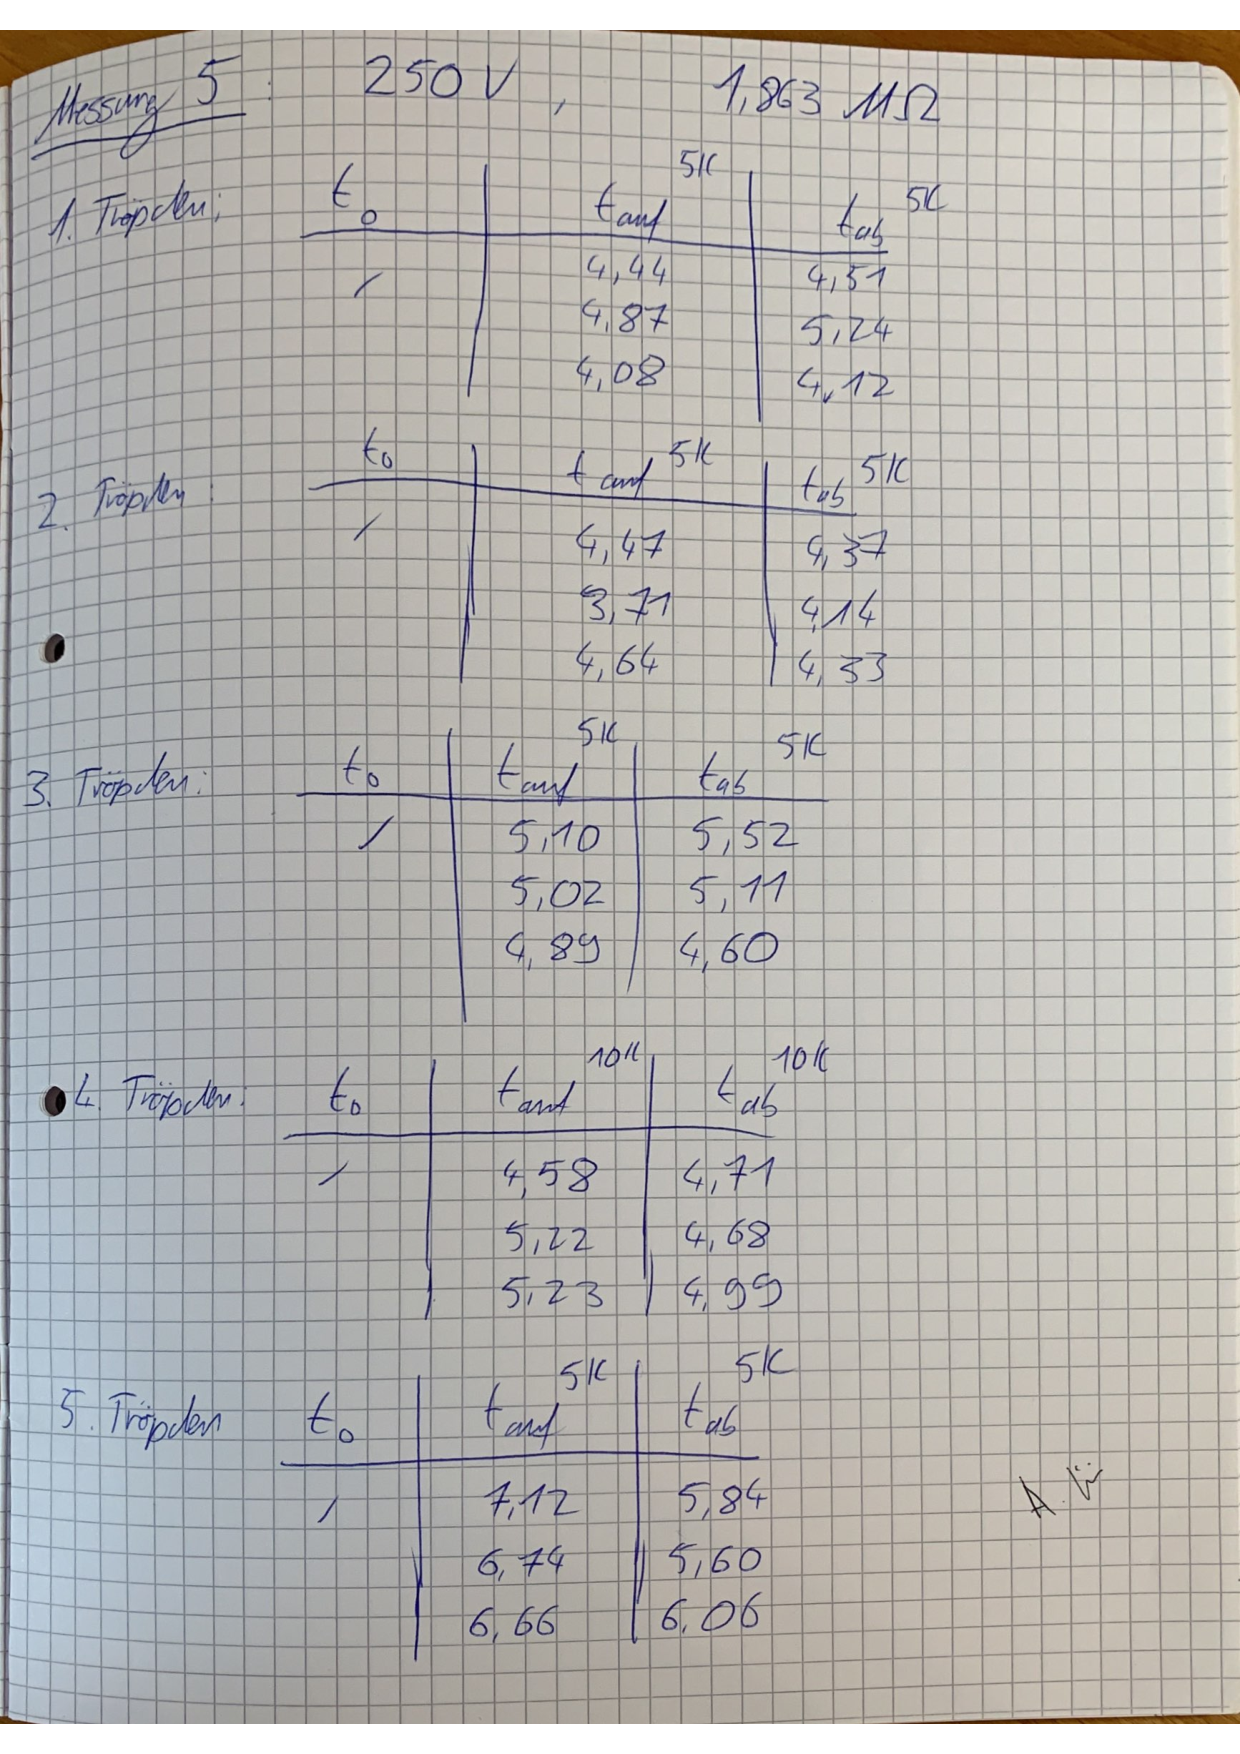
\includegraphics[height=18cm]{content/pics/originaldaten/Originaldaten_5.pdf}

\subsection{Tabelle zur Bestimmung der freigesetzten Ladungen}

\begin{longtable}{c c c c}
    \caption{Tabellarische Darstellung der freigesetzten Ladungen.} \label{tab:Ladungen} \\
    \hline
    {$U \mathbin{/} \unit{\volt}$} & {$N \mathbin{/} {\unit{\second}}$} & {$I \mathbin{/} \unit{\micro\ampere}$} & {$Q \mathbin{/} \unit{\giga\electronvolt}$} \\
    \hline
    \endfirsthead
    \caption[]{Tabellarische Darstellung der freigesetzten Ladungen.(Fortsetzung)}\\
    \hline
    {$U \mathbin{/} \unit{\volt}$} & {$N \mathbin{/} {\unit{\second}}$} & {$I \mathbin{/} \unit{\micro\ampere}$} & {$Q \mathbin{/} \unit{\giga\electronvolt}$} \\
    \hline
    \endhead
    \hline
    \endfoot
    330  & $\num{ 82.33+-0.83}$ & 0,1 & $\num{ 7.6+-7.6}$ \\
    340  & $\num{ 83.28+-0.83}$ & 0,2 & $\num{15.0+-7.5}$ \\
    350  & $\num{ 85.17+-0.84}$ & 0,2 & $\num{14.7+-7.3}$ \\
    360  & $\num{ 84.66+-0.84}$ & 0,2 & $\num{14.7+-7.4}$ \\
    370  & $\num{ 86.61+-0.85}$ & 0,2 & $\num{14.4+-7.2}$ \\
    380  & $\num{ 86.05+-0.85}$ & 0,2 & $\num{14.5+-7.3}$ \\
    390  & $\num{ 87.03+-0.85}$ & 0,2 & $\num{14.3+-7.2}$ \\
    400  & $\num{ 87.63+-0.85}$ & 0,3 & $\num{21.4+-7.1}$ \\
    410  & $\num{ 87.14+-0.85}$ & 0,3 & $\num{21.5+-7.2}$ \\
    420  & $\num{ 89.33+-0.86}$ & 0,4 & $\num{27.9+-7.0}$ \\
    430  & $\num{114.33+-0.98}$ & 0,4 & $\num{21.8+-5.5}$ \\
    440  & $\num{136.47+-1.07}$ & 0,4 & $\num{18.3+-4.6}$ \\
    450  & $\num{136.38+-1.07}$ & 0,4 & $\num{18.3+-4.6}$ \\
    460  & $\num{132.77+-1.05}$ & 0,4 & $\num{18.8+-4.7}$ \\
    470  & $\num{117.57+-0.99}$ & 0,4 & $\num{21.2+-5.3}$ \\
    480  & $\num{ 89.89+-0.87}$ & 0,5 & $\num{34.7+-7.0}$ \\
    490  & $\num{ 88.38+-0.86}$ & 0,5 & $\num{35.3+-7.1}$ \\
    500  & $\num{ 87.94+-0.86}$ & 0,5 & $\num{35.5+-7.1}$ \\
    510  & $\num{ 88.02+-0.86}$ & 0,5 & $\num{35.5+-7.1}$ \\
    520  & $\num{ 88.47+-0.86}$ & 0,6 & $\num{42.3+-7.1}$ \\
    530  & $\num{ 91.58+-0.87}$ & 0,6 & $\num{40.9+-6.8}$ \\
    540  & $\num{100.38+-0.91}$ & 0,6 & $\num{37.3+-6.2}$ \\
    550  & $\num{112.99+-0.97}$ & 0,6 & $\num{33.1+-5.5}$ \\
    560  & $\num{109.84+-0.96}$ & 0,6 & $\num{34.1+-5.7}$ \\
    570  & $\num{ 89.16+-0.86}$ & 0,6 & $\num{42.0+-7.0}$ \\
    580  & $\num{ 88.12+-0.86}$ & 0,6 & $\num{42.5+-7.1}$ \\
    590  & $\num{ 89.83+-0.87}$ & 0,6 & $\num{41.7+-7.0}$ \\
    600  & $\num{ 88.90+-0.86}$ & 0,7 & $\num{49.1+-7.0}$ \\
    610  & $\num{ 88.52+-0.86}$ & 0,7 & $\num{49.4+-7.1}$ \\
    620  & $\num{ 88.42+-0.86}$ & 0,7 & $\num{49.4+-7.1}$ \\
    630  & $\num{ 90.48+-0.87}$ & 0,7 & $\num{48.3+-6.9}$ \\
    640  & $\num{ 88.67+-0.86}$ & 0,7 & $\num{49.3+-7.1}$ \\
    650  & $\num{ 89.67+-0.86}$ & 0,7 & $\num{48.7+-7.0}$ \\
    660  & $\num{ 90.65+-0.87}$ & 0,8 & $\num{55.1+-6.9}$ \\
    670  & $\num{ 89.78+-0.86}$ & 0,8 & $\num{55.6+-7.0}$ \\
    680  & $\num{ 89.39+-0.86}$ & 0,8 & $\num{55.9+-7.0}$ \\
    690  & $\num{ 91.71+-0.87}$ & 0,8 & $\num{54.4+-6.8}$ \\
    700  & $\num{ 93.00+-0.88}$ & 0,8 & $\num{53.7+-6.7}$ \\
    \bottomrule
\end{longtable}